%%%%%%%%%%%%%%%%%%%%%%%%%%%%%%%%%%%%%%%%%
% Beamer Presentation
% LaTeX Template
% Version 1.0 (10/11/12)
%
% This template has been downloaded from:
% http://www.LaTeXTemplates.com
%
% License:
% CC BY-NC-SA 3.0 (http://creativecommons.org/licenses/by-nc-sa/3.0/)
%
%%%%%%%%%%%%%%%%%%%%%%%%%%%%%%%%%%%%%%%%%

%----------------------------------------------------------------------------------------
%   PACKAGES AND THEMES
%----------------------------------------------------------------------------------------

%\documentclass{beamer}
\documentclass[aspectratio=169]{beamer}
\mode<presentation> {

  % The Beamer class comes with a number of default slide themes
  % which change the colors and layouts of slides. Below this is a list
  % of all the themes, uncomment each in turn to see what they look like.

  %\usetheme{default}
  %\usetheme{AnnArbor}
  %\usetheme{Antibes}
  %\usetheme{Bergen}
  %\usetheme{Berkeley}
  %\usetheme{Berlin}
  %\usetheme{Boadilla}
  %\usetheme{CambridgeUS}
  %\usetheme{Copenhagen}
  %\usetheme{Darmstadt}
  %\usetheme{Dresden}
  %\usetheme{Frankfurt}
  %\usetheme{Goettingen}
  %\usetheme{Hannover}
  %\usetheme{Ilmenau}
  %\usetheme{JuanLesPins}
  %\usetheme{Luebeck}
  \usetheme{Madrid}
  %\usetheme{Malmoe}
  %\usetheme{Marburg}
  %\usetheme{Montpellier}
  %\usetheme{PaloAlto}
  %\usetheme{Pittsburgh}
  %\usetheme{Rochester}
  %\usetheme{Singapore}
  %\usetheme{Szeged}
  %\usetheme{Warsaw}

  % As well as themes, the Beamer class has a number of color themes
  % for any slide theme. Uncomment each of these in turn to see how it
  % changes the colors of your current slide theme.

  %\usecolortheme{albatross}
  %\usecolortheme{beaver}
  %\usecolortheme{beetle}
  %\usecolortheme{crane}
  %\usecolortheme{dolphin}
  %\usecolortheme{dove}
  %\usecolortheme{fly}
  %\usecolortheme{lily}
  %\usecolortheme{orchid}
  %\usecolortheme{rose}
  %\usecolortheme{seagull}
  %\usecolortheme{seahorse}
  \usecolortheme{whale}
  %\usecolortheme{wolverine}

  %\setbeamertemplate{footline} % To remove the footer line in all slides uncomment this line
  %\setbeamertemplate{footline}[page number] % To replace the footer line in all slides with a simple slide count uncomment this line

  %\setbeamertemplate{navigation symbols}{} % To remove the navigation symbols from the bottom of all slides uncomment this line
}
\usefonttheme[onlymath]{serif}
%\usepackage{epsfig}
\usepackage{amsmath}
\usepackage{graphicx} % Allows including images
\usepackage{booktabs} % Allows the use of \toprule, \midrule and \bottomrule in tables
\usepackage{multimedia} % 
%\usepackage{animate}
%\usepackage{tikz}
%\usepackage{lipsum}

\usepackage{tikz} 
\usetikzlibrary{tikzmark,overlay-beamer-styles,positioning,calc}
%\usetikzlibrary{tikzmark,
%\usetikzlibrary{tikzmark}
%\usetikzlibrary{arrows,shapes}
%\newcommand{\tikzmark}[1]{\tikz[remember picture] \node[coordinate] (#1) {#1};}
\newcommand{\be}{\begin{equation*}}
\newcommand{\ee}{\end{equation*}}
\newcommand{\ol}{\overline}
\newcommand{\p}{\partial}
\newcommand{\pdv}[2]{\frac{\partial \, #1}{\partial #2}}
\newcommand{\etal}{ {\it et al.} }
%----------------------------------------------------------------------------------------
%   TITLE PAGE
%----------------------------------------------------------------------------------------

\title[CHARTS]{Candidate CHARTS Model Update} % The short title appears at the bottom of every slide, the full title is only on the title page

\author[]{Brad Johnson\\Liz Holzenthal\\Rusty Permenter \\Kevin Hodgens } % Your name
\institute[ERDC] % Your institution as it will appear on the bottom of every slide, may be shorthand to save space
{USACE Engineering Research and Devlelopment Center \\ % Your institution for the title page
\medskip
\textit{} % Your email address
}
%\date{\today} % Date, can be changed to a custom date
\date{\vspace*{-0cm}\\ Nov, 2024} % Date, can be changed to a custom date

\begin{document}

\begin{frame}
  %\titlepage % Print the title page as the first slide
  \begin{columns}[c] % The "c" option specifies centered vertical alignment while the "t" option is used for top vertical alignment
    
    \column{.3\textwidth} % Left column and width
    \titlepage % Print the title page as the first slide
%%     \vspace*{-1cm}
%%     \begin{center}
%% District PDT:\\
%% Kelly Legault (SAJ)\\
%% Gabriel Todaro (SAJ)
%%     \end{center}
    \column{.7\textwidth} % Right column and width
    \begin{figure}
            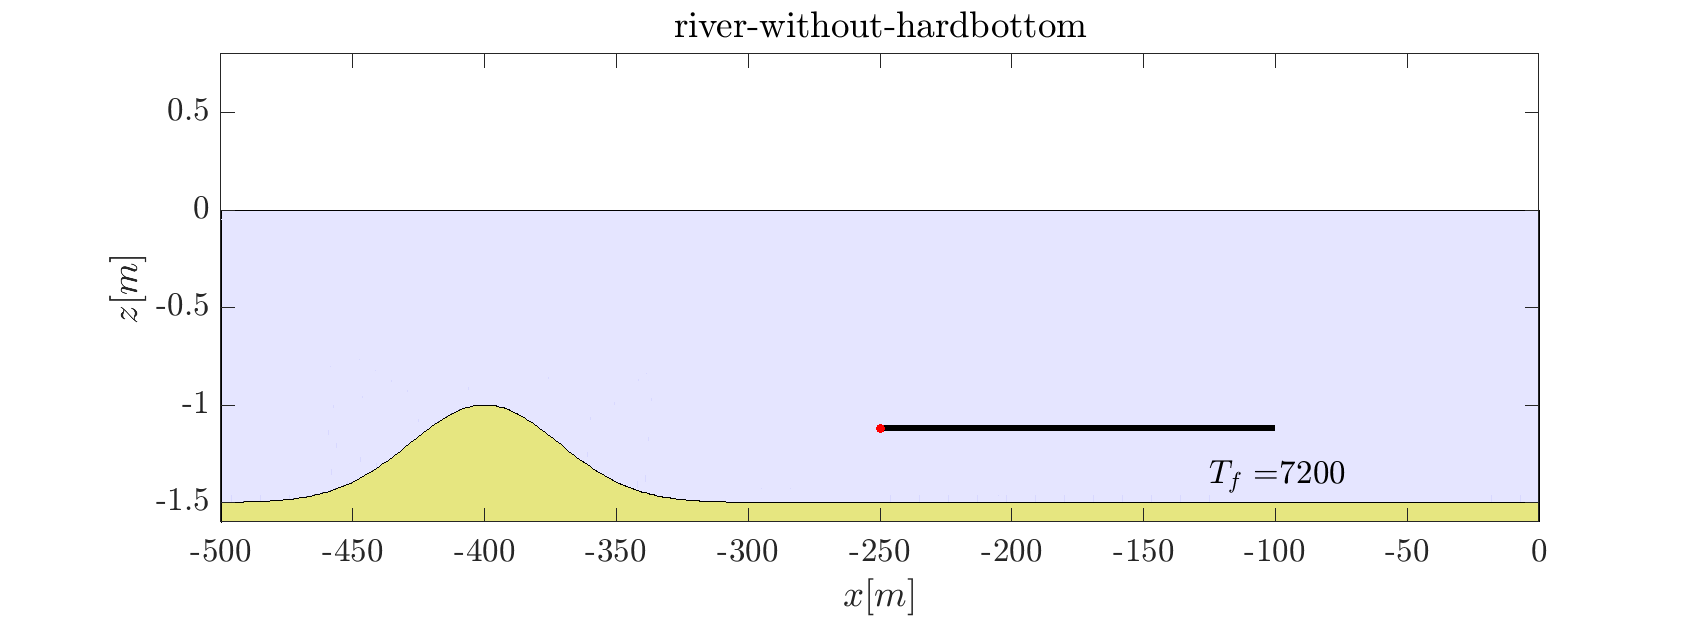
\includegraphics[width=1\linewidth]{../../graphics/river_without_hardbottom.png}
      %\includegraphics[trim={0 1cm 0 0},clip,width=0.9\linewidth]{./breaking-wave-on-the-beach.jpg}
    \end{figure}
    
  \end{columns}
\end{frame}
%%%%%%%%%%%%%%%%%%%%%%%%%%%%%%%%%%%%%%%%%%%%%%%%%%%%%%%%%%%%%%%%%%%%%%%%%%%%%%%%%%%%%%%%%%%%%%%%%%%%

\begin{frame}
  \frametitle{Model Review}
Previous presentation introduced simple, stable, and computationally efficient hydrodynamics framework:
 \begin{columns}[c] % 
    
   \column{.5\textwidth} % Left column and width

 \begin{itemize}
 \item One-dimensional
 \item Phase-averaged but low-frequency resolving
 \item Based on NLSW 
 \item Heuristic wet/dry
 \item Emphasis on simple and efficient
 \item Limited options for 'ocean' and 'landward' BC
 \item No transport 
   \end{itemize}
   \column{.5\textwidth} % Left column and width
    \begin{figure}
      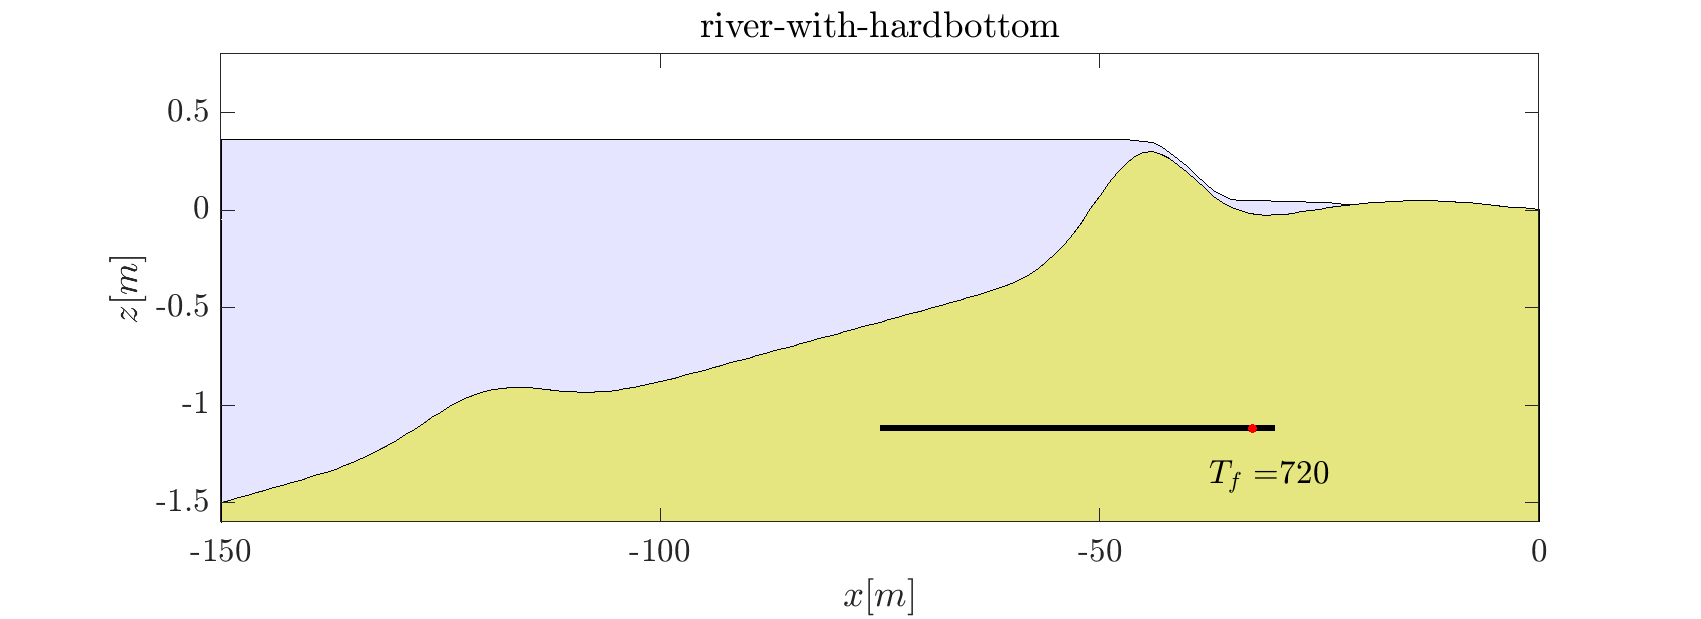
\includegraphics[width=1\linewidth]{./present.png}
    \end{figure}

 \end{columns}
 \end{frame}
%%%%%%%%%%%%%%%%%%%%%%%%%%%%%%%%%%%%%%%%%%%%%%%%%%%%%%%%%%%%%%%%%%%%%%%%%%%%%%%%%%%%%%%%%%%%%%%%%%%%
\begin{frame}
  \frametitle{New BC option}
  Model now permits the specification of $\eta$ on both ocean and bay sides, here with phase-lagged 'tide' and waves propagating in $+x$
 % \centering
  \movie[externalviewer]{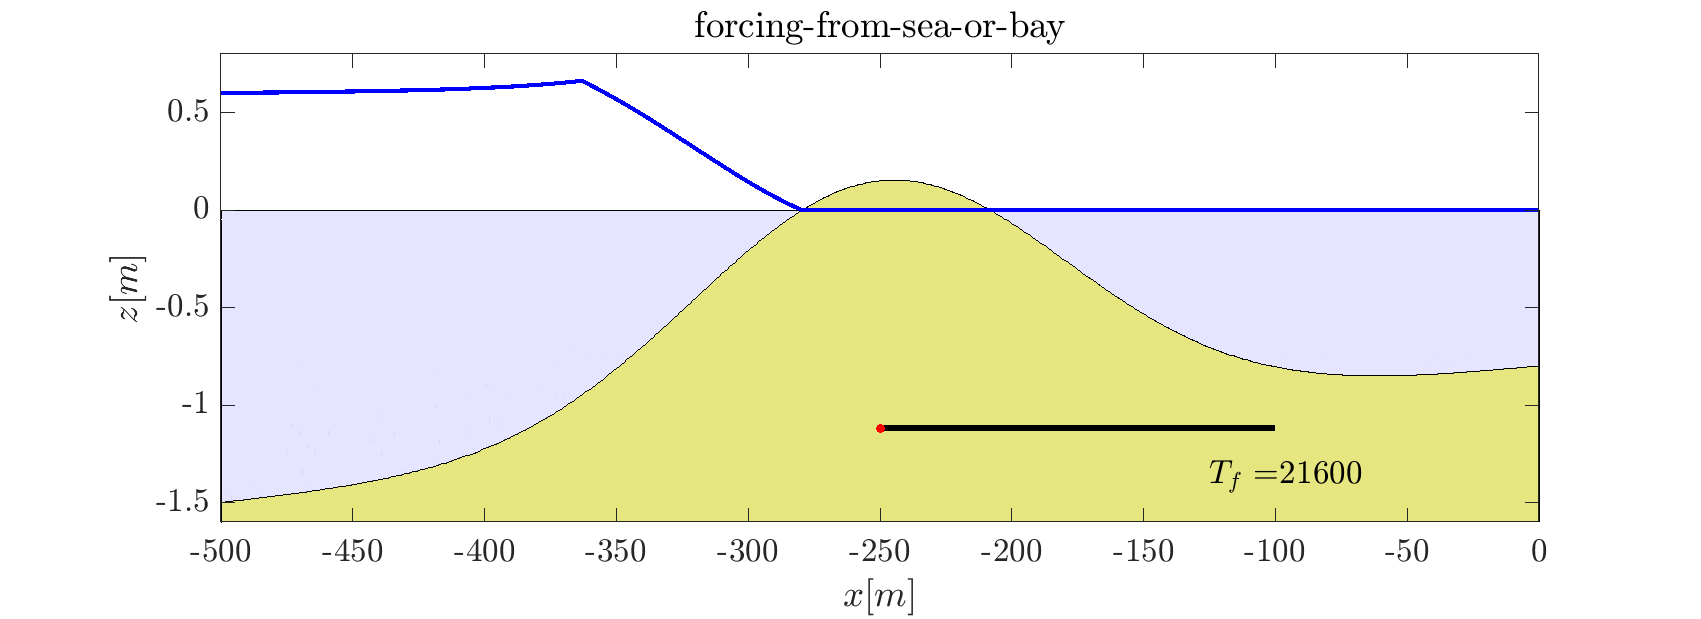
\includegraphics[width=\textwidth, keepaspectratio]
    {../../graphics/forcing_from_sea_or_bay.png}}{../../graphics/forcing_from_sea_or_bay.avi}
\end{frame}
%%%%%%%%%%%%%%%%%%%%%%%%%%%%%%%%%%%%%%%%%%%%%%%%%%%%%%%%%%%%%%%%%%%%%%%%%%%%%%%%%%%%%%%%%%%%%%%%%%%%
\begin{frame}
  \frametitle{Characterizing Bottom Shear }

In keeping with the simple/efficient model objective, the first
transport is formulated as an equilibrium energetics type, requiring
shear estimates.

Instantaneous skin friction is expressed with quadratic shear
\begin{equation*}
\tau_s = \rho c_f |u|u 
\end{equation*}
where total velocity, $u = U_{NLSW} + U_r + \tilde{u} $ is comprised
of a NLSW model current, a depth-averaged wave mass flux return current,
and a wave component, respectively.  The return current is expressed as a balance of the linear mass flux:
\begin{equation*}
U_r =   \frac{g H^2}{8 c h}
\end{equation*}
\end{frame}
%%%%%%%%%%%%%%%%%%%%%%%%%%%%%%%%%%%%%%%%%%%%%%%%%%%%%%%%%%%%%%%%%%%%%%%%%%%%%%%%%%%%%%%%%%%%%%%%%%%%
\begin{frame}
  \frametitle{Wave-Related Velocities}
  The impact of a skewed wave-form is admitted in the model with a 
  near-bed velocity time-series represented as a fundamental sinusoidal component and the phase-locked first harmonic, 

  \begin{columns}[c] % 
    
   \column{.5\textwidth} % Left column and width
\begin{equation*}
\tilde{u} = U_0 \cos{\omega t}+ U_1 \cos{2 \omega t}
\end{equation*}
  where
 \begin{align*}
   \sigma_u &= \frac{\sigma_{\eta} \omega}{ \sinh{kh}} = \frac{H \omega}{\sqrt{8} \sinh{kh}}\\
   U_0 &= \frac{ \sqrt{2} \sigma_u}{\sqrt{1+S^2}}\\
   U_1 &= S U_0
 \end{align*}
 where $S$ is an empirical skewness param ranging from $0 \rightarrow ~1/2$.
 \column{.5\textwidth} % Left column and width
 \begin{figure}
   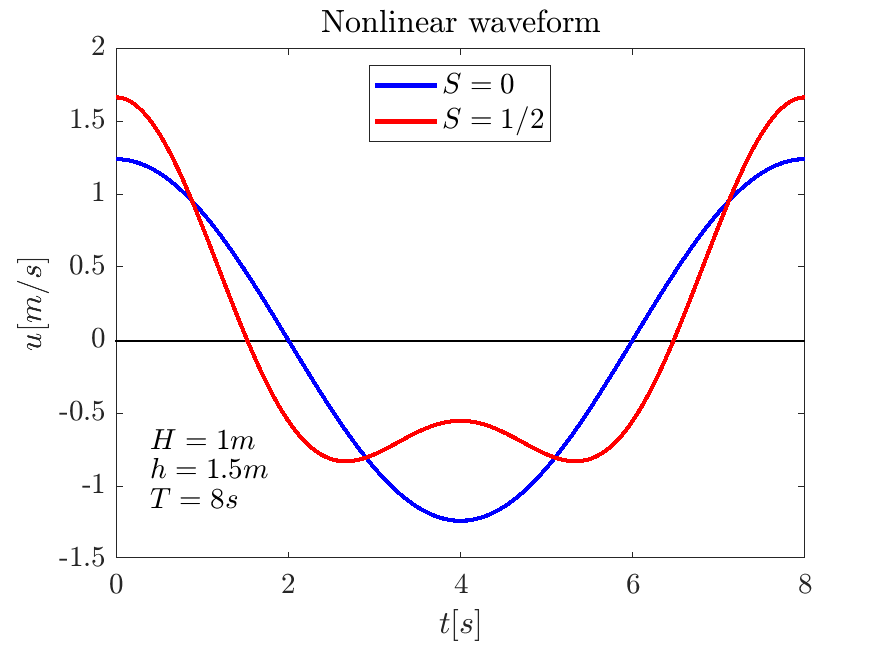
\includegraphics[width=1\linewidth]{./skewness.png}
 \end{figure}
  \end{columns} 
 \end{frame}
%%%%%%%%%%%%%%%%%%%%%%%%%%%%%%%%%%%%%%%%%%%%%%%%%%%%%%%%%%%%%%%%%%%%%%%%%%%%%%%%%%%%%%%%%%%%%%%%%%%%
\begin{frame}
  \frametitle{Equilibrium Transport Model}

  Equilibrium models are appropriate for regions of slowly varied bed
  and hydrodynamic forcing, and the following is based on an
  excess-shear energetics approach.

\begin{equation*}
  q_{eq} = 8 B \sqrt{g (s-1) d_{50}^3}(\theta-\theta_{cr})^{3/2} \;\;\; \mbox{for} \;\; \theta>\theta_{cr}
\end{equation*}
where
\begin{align*}
  \theta &= \frac{\tau_s}{\rho g (s-1) d_{50}} \;\;\;\; ; \;\;\;  \theta_{cr} \simeq 0.05
\end{align*}
and $B$ is an empirical param with $B=1$ corresponding to the
Meyer-Peter and Müller model.

\end{frame}
%%%%%%%%%%%%%%%%%%%%%%%%%%%%%%%%%%%%%%%%%%%%%%%%%%%%%%%%%%%%%%%%%%%%%%%%%%%%%%%%%%%%%%%%%%%%%%%%%%%%
\begin{frame}
  \frametitle{Equilibrium Transport Model}


Recall that the shear has both wave and
current components, so time-averaging is done with a synthetic wave-current time-series and numerical summation

\begin{equation*}
  \overline{q_{eq}} = \frac{8 B}{T} \sqrt{g (s-1) d_{50}^3}\int_0^T(\theta(t)-\theta_{cr})^{3/2} dt 
\end{equation*}

Bottom evolution is dictated by conservation of sand
\begin{equation*}
\pdv{z_b}{t} = -\frac{1}{1-n} \pdv{\overline{q_{eq}}}{x}
\end{equation*}
where $n$ is the bed porosity, which is solved numerically for the bed
evolution in time with an first-order time-explicit scheme with
second-order central differences in space.


\end{frame}
%%%%%%%%%%%%%%%%%%%%%%%%%%%%%%%%%%%%%%%%%%%%%%%%%%%%%%%%%%%%%%%%%%%%%%%%%%%%%%%%%%%%%%%%%%%%%%%%%%%%
\begin{frame}
  \frametitle{Equilibrium Transport Model for River} 
  \centering
  \movie[externalviewer]{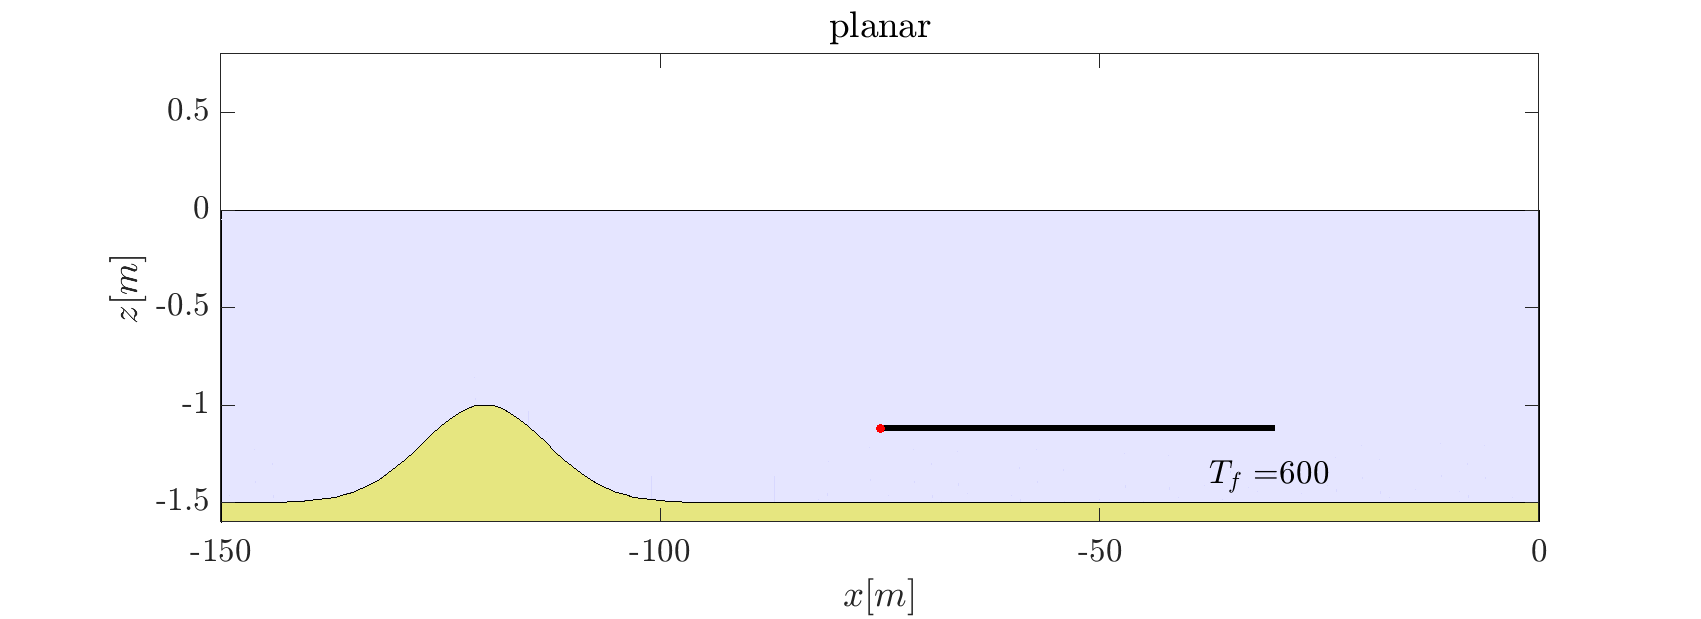
\includegraphics[width=\textwidth, keepaspectratio]
    {../../graphics/river_equilibrium.png}}{../../graphics/river_equilibrium.avi}
\end{frame}
%%%%%%%%%%%%%%%%%%%%%%%%%%%%%%%%%%%%%%%%%%%%%%%%%%%%%%%%%%%%%%%%%%%%%%%%%%%%%%%%%%%%%%%%%%%%%%%%%%%%
\begin{frame}
  \frametitle{Equilibrium Transport Model Without Waves} 
  \centering
  \movie[externalviewer]{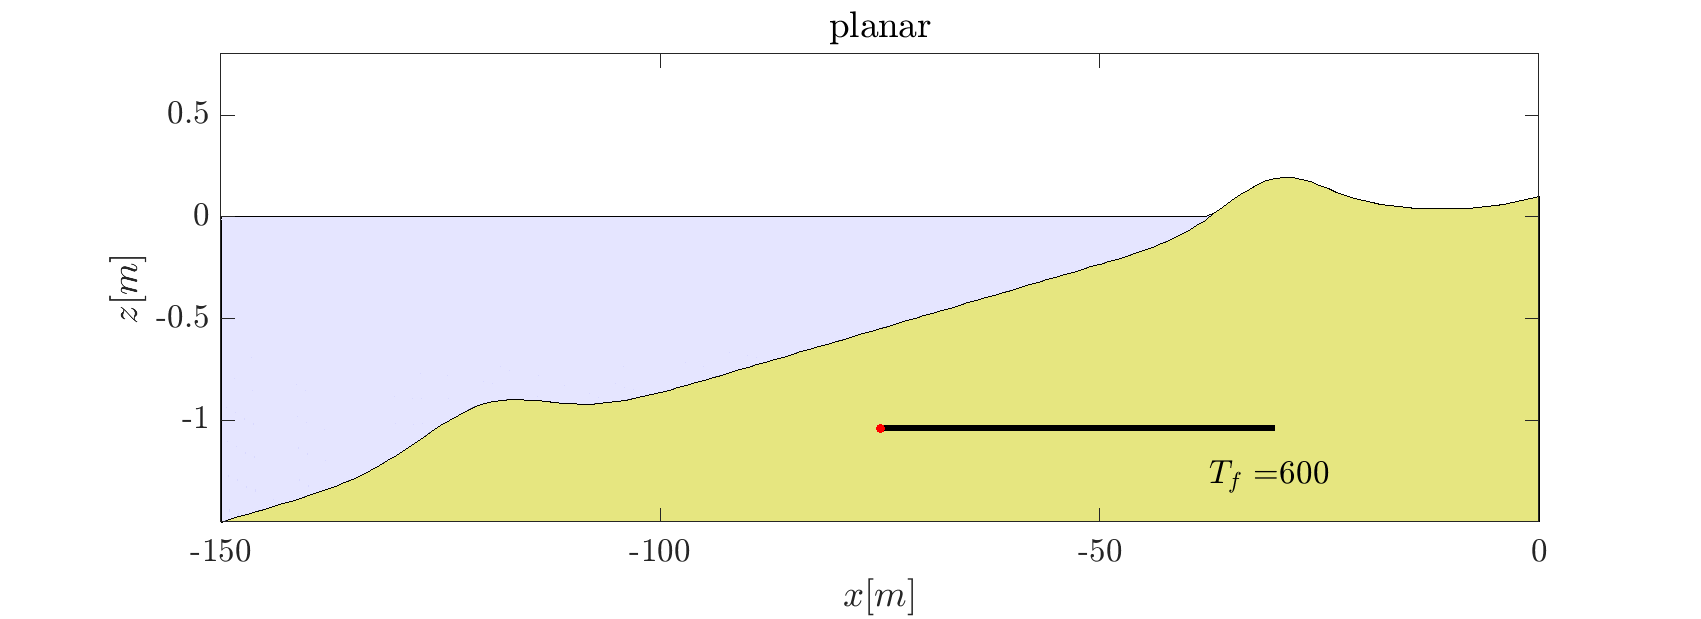
\includegraphics[width=\textwidth, keepaspectratio]
    {../../graphics/overwash_without_waves.png}}{../../graphics/overwash_without_waves.avi}
\end{frame}
%%%%%%%%%%%%%%%%%%%%%%%%%%%%%%%%%%%%%%%%%%%%%%%%%%%%%%%%%%%%%%%%%%%%%%%%%%%%%%%%%%%%%%%%%%%%%%%%%%%%
\begin{frame}
  \frametitle{Equilibrium Transport Model With Waves} 
  \centering
  \movie[externalviewer]{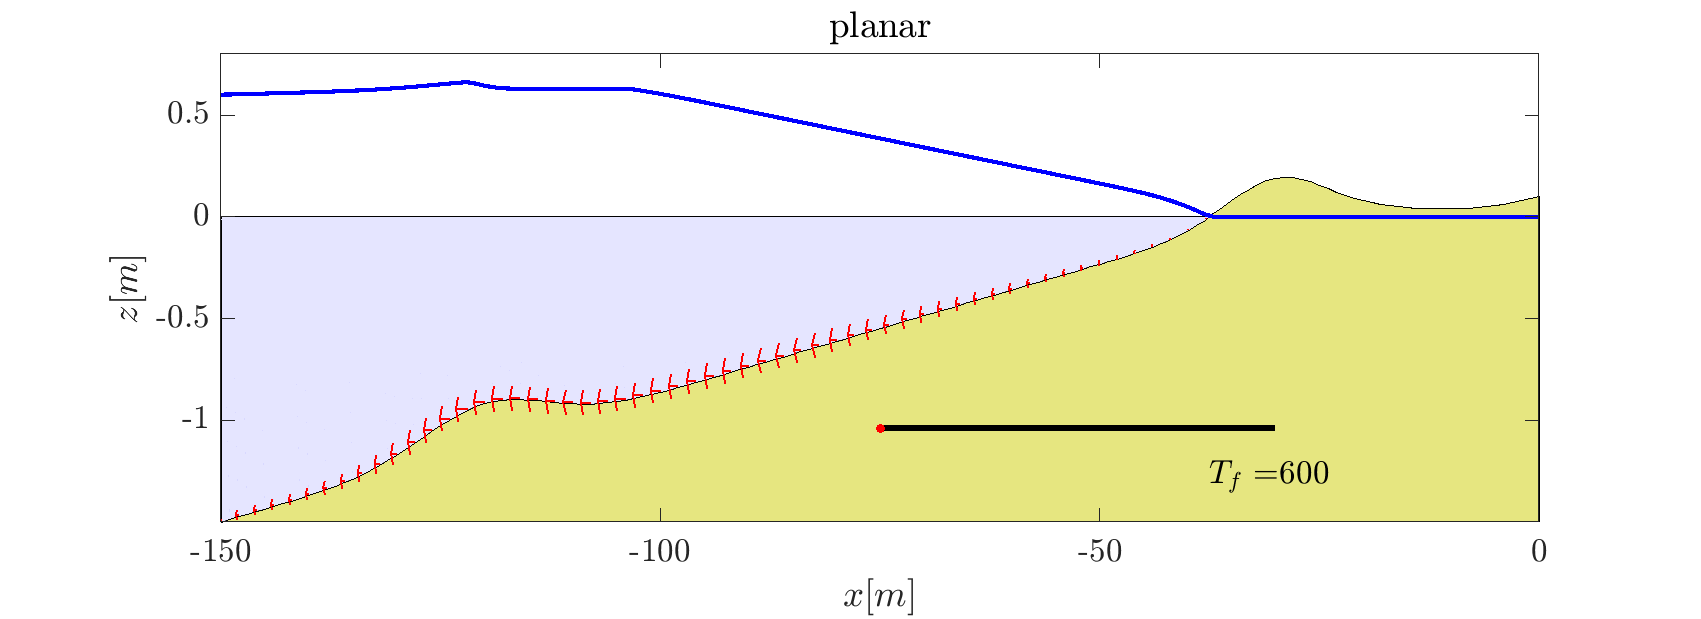
\includegraphics[width=\textwidth, keepaspectratio]
    {../../graphics/overwash_with_waves.png}}{../../graphics/overwash_with_waves.avi}
\end{frame}
%%%%%%%%%%%%%%%%%%%%%%%%%%%%%%%%%%%%%%%%%%%%%%%%%%%%%%%%%%%%%%%%%%%%%%%%%%%%%%%%%%%%%%%%%%%%%%%%%%%%
\begin{frame}
  \frametitle{Non-Equilibrium Transport Model} Of course, it is not
  always realistic to assume that the transport is in balance with the
  forcing owing to gradients in
  \begin{itemize}
  \item Temporal: Waves, in particular, can generate transport in
    disequilibrium owing to the rapid variation of the wave orbital
    velocity components.  This is particularly true of the suspended
    transport that can exhibit temporal lag between forcing and
    response.  I have not approached this issue at present as the
    previously introduced transport formulation is more consistent
    with a bedload algorithm, which, conventionally, is assumed to
    react instantaneously.
  \item 
    Spatial: In the presence of pronounced variation in either forcing
    or sediment characteristics, transport can demonstrate significant
    departures from the equilibrium estimates.  Of particular
    importance are cases that have limitations in sediment
    availability such as domains that have a combination of sand bed
    and hard-bottom.
  \end{itemize}
\end{frame}
%%%%%%%%%%%%%%%%%%%%%%%%%%%%%%%%%%%%%%%%%%%%%%%%%%%%%%%%%%%%%%%%%%%%%%%%%%%%%%%%%%%%%%%%%%%%%%%%%%%%
\begin{frame}
  \frametitle{Non-Equilibrium Transport Model} 

  Accounting for spatial gradients is achieved by equating gradients
  in transport $q$ and bed-pickup $P$ and fallout, $F$

  \begin{equation*}
    \pdv{\overline{q}}{x} = P-F 
  \end{equation*}
Fallout $F$ can be expressed in terms of near-bed concentration, $c$
as $F = w_f c = \frac{w_f}{u \delta} \overline{q} $ which makes use of
$q = u \delta c$ where $\delta$ is a bedload layer thickness $\sim 0.01m$.
Similarly, the pickup, $P = A \frac{w_f}{u \delta} \overline{q_{eq}}$
where $A$ is a modifier equal to 0 or 1 indicating the availability of sand in the bed
to be suspended.  Note that the formulation can also be represented with a disequilibrium model 
  \begin{equation*}
    \pdv{\overline{q}}{x} = \frac{A \overline{q_{eq}}  - \overline{q}}{L} \;\;\;\;\mbox{where}\;\;\; L = \frac{u \delta}{w_f}
  \end{equation*}
and $L$ has the physical interpretation of a horizontal advection
length that a particle travels while falling through the
boundary layer.


  


\end{frame}
%%%%%%%%%%%%%%%%%%%%%%%%%%%%%%%%%%%%%%%%%%%%%%%%%%%%%%%%%%%%%%%%%%%%%%%%%%%%%%%%%%%%%%%%%%%%%%%%%%%%
\begin{frame}
  \frametitle{Non-Equilibrium Transport Model} To demonstrate the
  numerical solution for the previously introduced expression for
  non-equilibrium transport, a FD statement is provided at node $i$:
  \begin{equation*}
    \frac{q_{i+1}-q_{i-1}}{2\Delta x} = \frac{w_f}{u_i \delta}\left\{ q_{eq_i} - q_i\right\} 
  \end{equation*}
constituting a linear expression in $q$ for nodes 2...N-1.  Presently,
boundaries are treated with a zero gradient with $q_1 = q_2$ and $q_N = q_{N-1}$ 

  \begin{equation*}
\begin{bmatrix}
-1 & 1                               & 0 & \\
-1 & 2\Delta x \frac{w_f}{u_2 \delta} & 1 & 0\\
0  & -1                              &2\Delta x \frac{w_f}{u_3 \delta}&1&0\\
&&&&\cdot\\
&&&&&\cdot\\
&&&&&-1&2\Delta x \frac{w_f}{u_{N-1} \delta}&1\\
&&&&&0 &-1&1\\
\end{bmatrix}
\begin{bmatrix}
  q_1\\
  q_2\\
  q_3\\
  \cdot\\
  \cdot\\
  q_{N-1}\\
    q_{N}
\end{bmatrix}
=
\begin{bmatrix}
  0\\
  A_2 2\Delta x \frac{w_f}{u_2 \delta}q_{eq_2}\\
  A_3 2\Delta x \frac{w_f}{u_2 \delta}q_{eq_3}\\
  \cdot\\
  \cdot\\
   A_{N-1} 2\Delta x \frac{w_f}{u_2 \delta}q_{eq_{N-1}}\\
  0
\end{bmatrix}
  \end{equation*}

\end{frame}
%%%%%%%%%%%%%%%%%%%%%%%%%%%%%%%%%%%%%%%%%%%%%%%%%%%%%%%%%%%%%%%%%%%%%%%%%%%%%%%%%%%%%%%%%%%%%%%%%%%%
\begin{frame}
  \frametitle{Non-Equilibrium Transport Model} 
  \centering
  \movie[externalviewer]{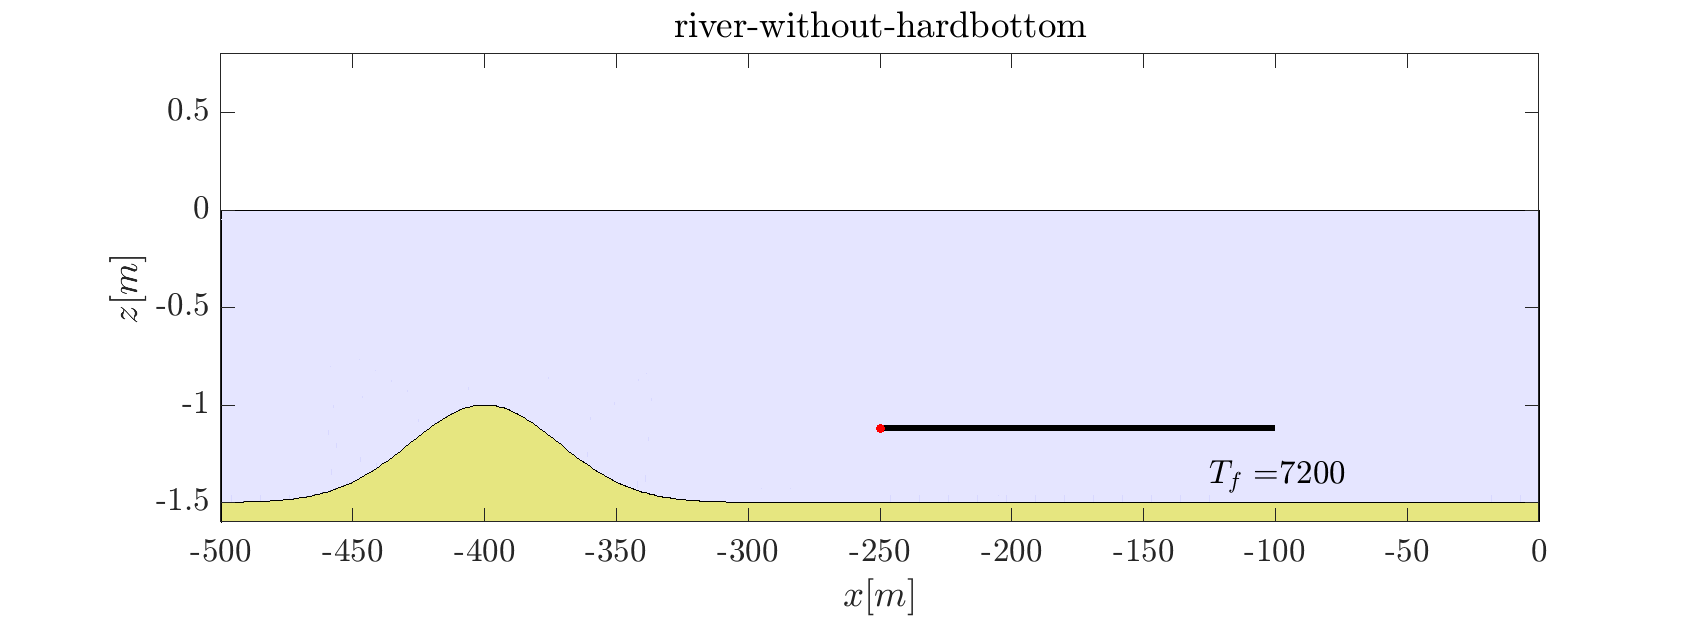
\includegraphics[width=\textwidth, keepaspectratio]
    {../../graphics/river_without_hardbottom.png}}{../../graphics/river_without_hardbottom.avi}
\end{frame}
%%%%%%%%%%%%%%%%%%%%%%%%%%%%%%%%%%%%%%%%%%%%%%%%%%%%%%%%%%%%%%%%%%%%%%%%%%%%%%%%%%%%%%%%%%%%%%%%%%%%
\begin{frame}
  \frametitle{Non-Equilibrium Transport Model} 
  \centering
  \movie[externalviewer]{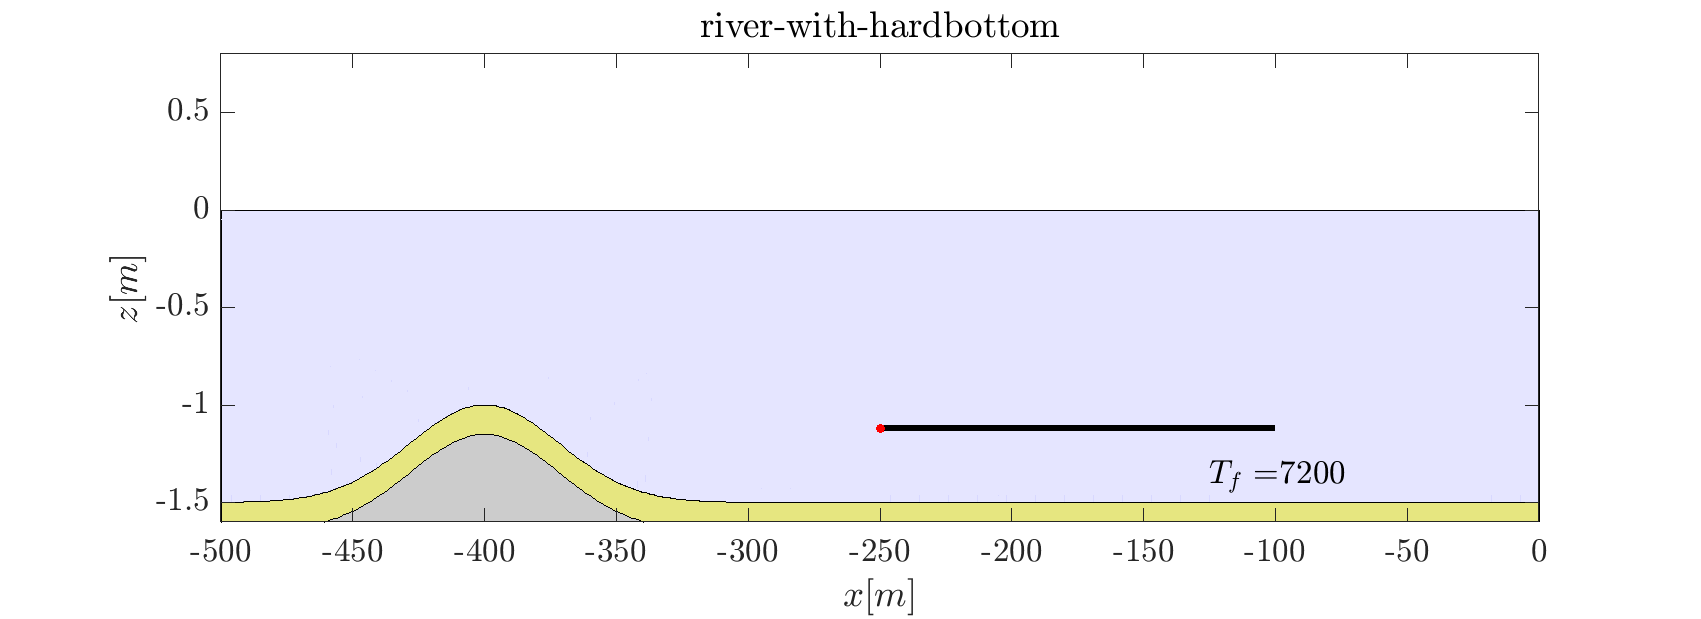
\includegraphics[width=\textwidth, keepaspectratio]
    {../../graphics/river_with_hardbottom.png}}{../../graphics/river_with_hardbottom.avi}
\end{frame}
%%%%%%%%%%%%%%%%%%%%%%%%%%%%%%%%%%%%%%%%%%%%%%%%%%%%%%%%%%%%%%%%%%%%%%%%%%%%%%%%%%%%%%%%%%%%%%%%%%%%
\begin{frame}
  \frametitle{Non-Equilibrium Transport Model} 
  \centering
  \movie[externalviewer]{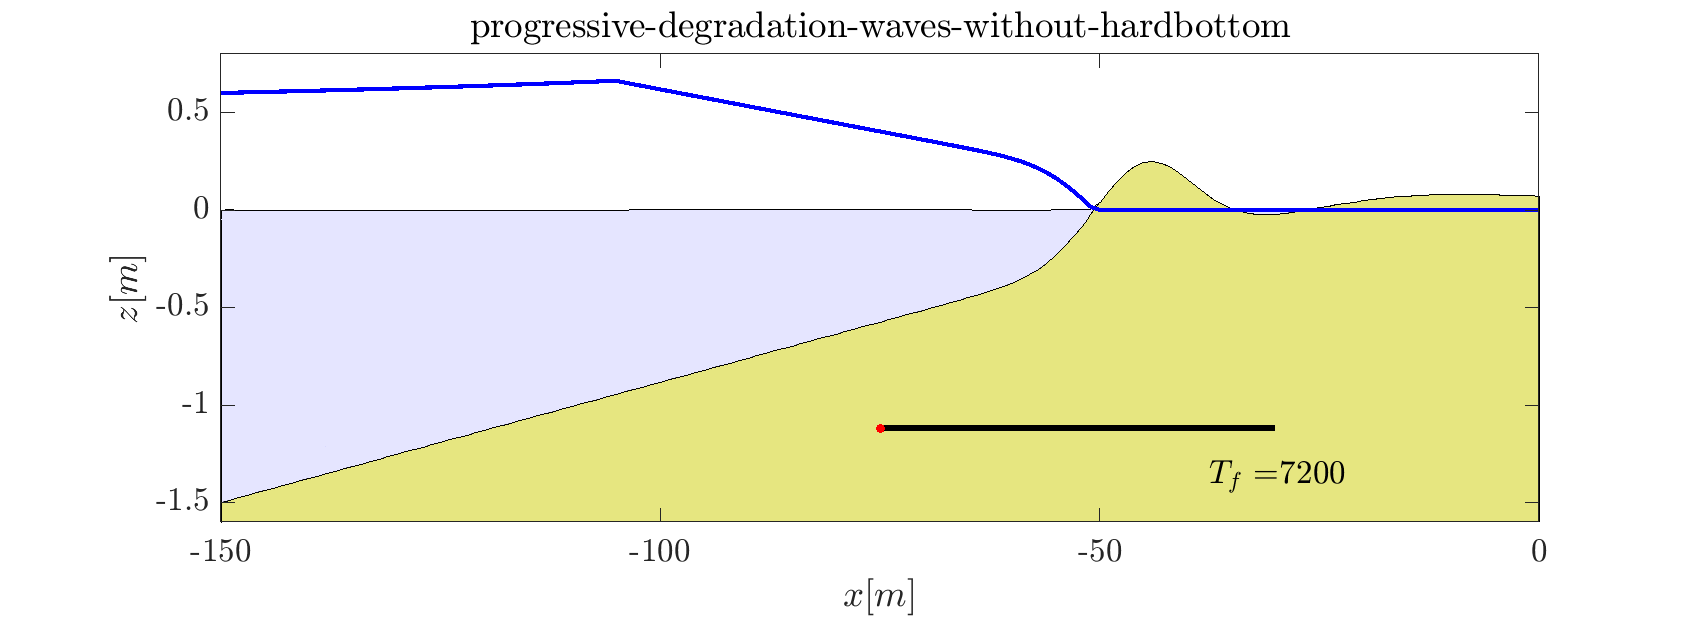
\includegraphics[width=\textwidth, keepaspectratio]
    {../../graphics/progressive_degradation_waves_without_hardbottom.png}}{../../graphics/progressive_degradation_waves_without_hardbottom.avi}
\end{frame}
%%%%%%%%%%%%%%%%%%%%%%%%%%%%%%%%%%%%%%%%%%%%%%%%%%%%%%%%%%%%%%%%%%%%%%%%%%%%%%%%%%%%%%%%%%%%%%%%%%%%
\begin{frame}
  \frametitle{Non-Equilibrium Transport Model} 
  \centering
  \movie[externalviewer]{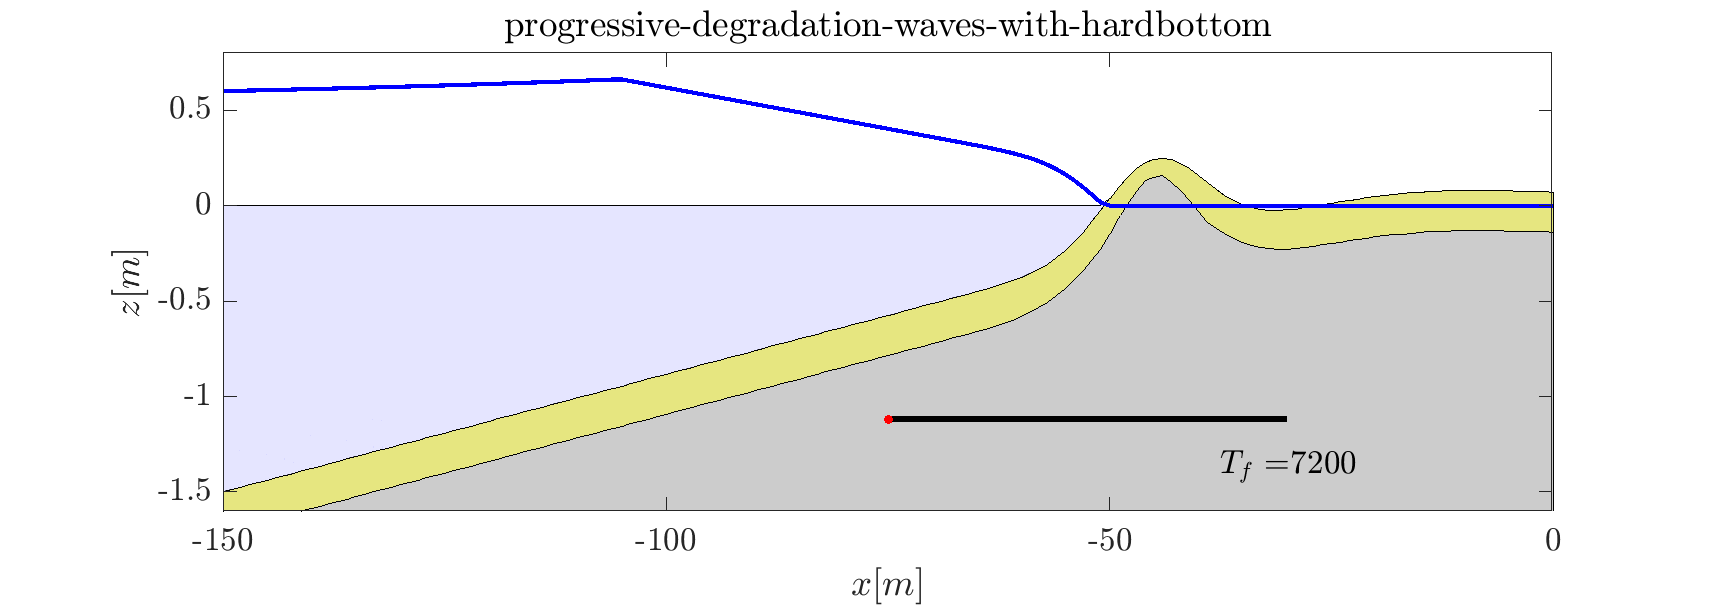
\includegraphics[width=\textwidth, keepaspectratio]
    {../../graphics/progressive_degradation_waves_with_hardbottom.png}}{../../graphics/progressive_degradation_waves_with_hardbottom.avi}
\end{frame}
%%%%%%%%%%%%%%%%%%%%%%%%%%%%%%%%%%%%%%%%%%%%%%%%%%%%%%%%%%%%%%%%%%%%%%%%%%%%%%%%%%%%%%%%%%%%%%%%%%%%
\begin{frame}
  \frametitle{Runtimes and Next Steps} 
Clock time for simulating 24 hrs 
\begin{center}
  \begin{tabular}{ |c|c|c| } 
    \hline
    $H$ & 50$s$ \\ 
    \hline
    $H+W$ & 200$s$ \\
    \hline
    $H+S_{eq}$ & 60$s$  \\
    \hline
    $H+S_{neq}$ & 440$s$  \\ 
    \hline
  \end{tabular}
\end{center}
Kill or Continue?

If we proceed, 
 \begin{itemize}
 \item Validate MSBC with Carrier and Greenspan?
 \item Develop suspended sed routine
 \item Validate sed transport or morphology ( implement some sort of testbed?)
 \item Start considering the union of the Storm/Quiescent periods
 \end{itemize}


\end{frame}
%%%%%%%%%%%%%%%%%%%%%%%%%%%%%%%%%%%%%%%%%%%%%%%%%%%%%%%%%%%%%%%%%%%%%%%%%%%%%%%%%%%%%%%%%%%%%%%%%%%%
\end{document}






